% Slide-n
\begin{frame}[t]{Point Estimation}
	The value of any statistic of any that estimates the value of a parameter 
	is called a point estimation. \\ 
	$\overline{x} = 2.9$ $\rightarrow$ $\mu = 3.00$
	
	We rarely know if our point estimate is correct because it is merely an 
	estimation of the actual value.
\end{frame}


\begin{frame}[t]{Confidence Interval}
	A Confidence Interval is a range of values we are fairly sure our true 
	value lies in. \\ 
	\begin{center}
		\begin{tabular}{|c|c|}
			\hline 
			Confidence Interval & Z-Value \\ 
			\hline 
			90\% & 1.65 \\ 
			\hline 
			95\% & 1.69 \\ 
			\hline 
			99\% & 2.58 \\ 
			\hline 
			99.9\% & 3.291 \\ 
			\hline 
		\end{tabular}
	\end{center}
\end{frame}

% Slide-n
\begin{frame}[t]{Calculating Confidence Intervals}
	We measure the heights of 40 randomly chosen men, and get a mean height of 
	175cm,We also know the standard deviation of men's heights is 20cm.
	
	\begin{itemize}
		\item \textbf{Step-1}
		\begin{itemize}
			\item[--]  the number of observations($n$)
			\item[--]  the mean $\overline{x}$
			\item[--] the standard deviation $s$
		\end{itemize}
		\item \textbf{Step-2:}
			\begin{itemize}
			\item[--]  number of observations n = 40
			\item[--]  mean X = 175
			\item[--]  standard deviation s = 20
		\end{itemize}
		\item \textbf{Step-3:} decide what Confidence Interval we want: 95\% or 
		99\% are common choices. Then find the "Z" value for that Confidence 
		\item \textbf{Step-4:} use that Z value in this formula for the 
		Confidence Interval.
		$$
		X \pm Z\frac{s}{\sqrt{n}}
		$$
	\end{itemize}
\end{frame}

% Slide-n
\begin{frame}[t]{Calculating Confidence Intervals}
	$$
	X \pm Z\frac{s}{\sqrt{n}}
	$$
	$$
	175\pm 1.960 \times \frac{20}{40} = 175cm\pm 6.20
	$$
\end{frame}

% Slide-n
\begin{frame}[t]{Bivariate Analysis}
	\begin{itemize}
		\item \textbf{Covariance:} Measures relationship between 
		two variables specially whether greater values of one variable 
		correspond to greater values in the other.
		\item \textbf{Correlation:} Similar to covariance; measures whether 
		greater values of one  variable correspond to greater values in the 
		other. Scaled to always lie between $+1$ and $-1$
	\end{itemize}
\end{frame}


% Slide-n
\begin{frame}[t]{Covariance}
	\begin{itemize}
		\item Covariance is a measure of how much two random variables vary 
		together.
		\item 	It’s similar to variance, but where variance tells you how a 
		single variable varies, covariance tells you how two variables vary 
		together.
	\end{itemize}

\begin{figure} [ht]
	\centering
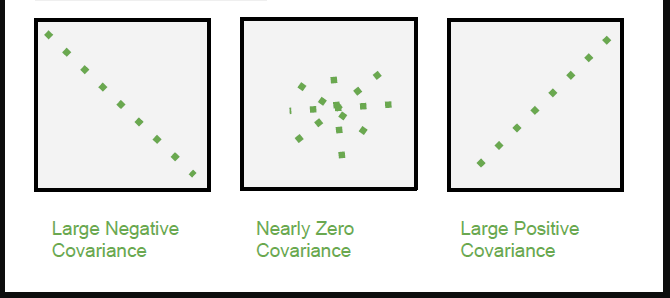
\includegraphics[trim={1cm 1cm 1cm 0}, clip, scale=0.4]{eda/cov.png}
	\source{https://www.statisticshowto.com/covariance/}
\end{figure}
	 
\end{frame}
% Slide-n
\begin{frame}[t]{Covariance}
	$$
	cov(x,y) = \frac{\sum{(x_i - \overline{x})(y_i - \overline{y})}}{n-1}	
	$$
	\begin{itemize}
		\item $cov(x,y)$ $\rightarrow$ covariance between $x$ and $y$
		\item $x_i$ $ \rightarrow$ data value of $x$
		\item $y_i$ $\rightarrow$ data value of $y$
		\item $\overline{x}$ $\rightarrow$  mean of $x$
		\item $\overline{y}$ $\rightarrow$ mean of $y$
		\item $n$ $\rightarrow$ number of data values. 
	\end{itemize}
	
	
\end{frame}

% Slide-n
\begin{frame}[t]{Correlation}
	\begin{itemize}
		\item When two sets of data are strongly linked together we say they 
		have a High Correlation.
		\item Correlation is \textbf{Positive} when the values increase 
		together.
		\item Correlation is \textbf{Negative} when one value decreases as the 
		other increases
		\item A correlation is assumed to be linear.	
	\end{itemize}

\begin{figure} [ht]
	\centering
	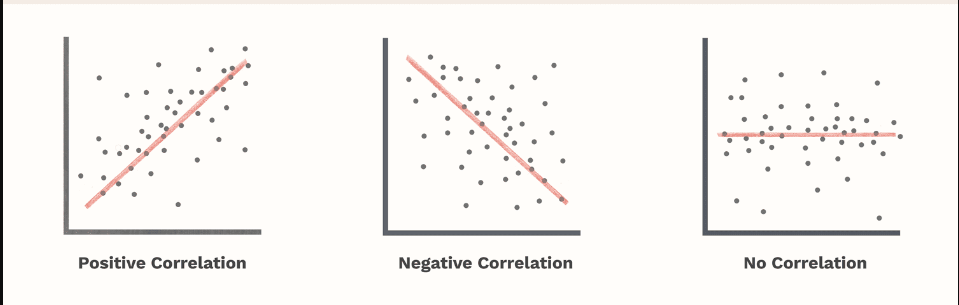
\includegraphics[trim={1cm 0cm 1cmcm 1cm}, clip, scale=0.4]{eda/corr}
\end{figure}
\end{frame}

% Slide-n
\begin{frame}[t]{Interpretation}
	\begin{itemize}
		\item 1 is a perfect positive correlation
		\item 0 is no correlation (the values don't seem linked at all)
		\item -1 is a perfect negative correlation
	\end{itemize}
\end{frame}

% Slide-n
\begin{frame}[t]{Pearson's r Correlation}
	\begin{itemize}
		\item  Pearson's $r$ measures the strength of the linear relationship 
		between two variables.
		\item Pearson's $r$ is always between -1 and 1 
	\end{itemize}
	
	\begin{equation*}
	r =
	\frac{ \sum_{i=1}^{n}(x_i-\bar{x})(y_i-\bar{y}) }{%
		\sqrt{\sum_{i=1}^{n}(x_i-\bar{x})^2}\sqrt{\sum_{i=1}^{n}(y_i-\bar{y})^2}}
	\end{equation*}



	\begin{itemize}
		\item $r$ $\rightarrow$ correlation between $x$ and $y$
		\item $x_i$ $ \rightarrow$ data value of $x$
		\item $y_i$ $\rightarrow$ data value of $y$
		\item $\overline{x}$ $\rightarrow$  mean of $x$
		\item $\overline{y}$ $\rightarrow$ mean of $y$
	\end{itemize}
\end{frame}

% Slide-n
\begin{frame}[t]{Correlation Is Not Causation}
	\begin{itemize}
		\item A common saying is "Correlation Is Not Causation".
		\item What it really means is that a correlation does not prove one 
		thing causes the other.
		\item Causation means that one variable causes something to happen in 
		another variable.
		\item To say that two things are correlated is to say that they are not 
		some kind of relationship.
		\item In order to imply causation, a true experiment must be performed 
		where subjects are randomly assigned to different conditions.
	\end{itemize}
\end{frame}
